\documentclass{article}
\usepackage{spikey}
\usepackage{amsmath}
\usepackage{mathrsfs}
\usepackage{amssymb}
\usepackage{soul}
\usepackage{float}
\usepackage{graphicx}
\usepackage{hyperref}
\usepackage{fancyhdr}
\usepackage{xcolor}
\usepackage{chngcntr}
\usepackage{centernot}
\usepackage[shortlabels]{enumitem}
\usepackage[margin=1truein]{geometry}
\usepackage{tkz-graph}
\usepackage{dsfont}
\usepackage{caption}
\usepackage{subcaption}

\usepackage{setspace}
\linespread{1.15}
\usepackage[margin=1truein]{geometry}

\counterwithin{equation}{section}
\counterwithin{figure}{section}

%\pagestyle{fancy}
%\lhead{Topics in Economics of Information}

\usepackage[
    type={CC},
    modifier={by-nc},
    version={4.0},
]{doclicense}

\title{CSC412/2506 Winter 2020: Probabilistic Learning and Reasoning}
\date{\today}
\author{Tianyu Du}
\begin{document}
    \maketitle
    \tableofcontents
    \newpage
    \section{Introduction}
    
    \section{Probabilistic Models}
	
	\begin{definition}
		Given an i.i.d. dataset $\mc{D}$, the log-likelihood of $\theta$ is defined as
		\begin{align}
			\ell(\theta;\mc{D}) = \sum_{i=1}^N \log p(x\upi|\theta)
		\end{align}
	\end{definition}
	
	\begin{definition}
		A \textbf{statistic} is a deterministic function of a set of random variables.
	\end{definition}
	
	\begin{definition}
		$T(X)$ is a \textbf{sufficient statistic} for random variable $X$ if
		\begin{align}
			T(x^{(1)}) = T(x^{(2)}) \implies L(\theta; x^{(1)}) = L(\theta; x^{(2)})\quad \forall \theta
		\end{align}
		equivalently,
		\begin{align}
			P(\theta|T(X)) = P(\theta|X)
		\end{align}
	\end{definition}
	
	\section{Directed Graphical Models}
	
	
	
	\subsection{Decision Theory}
	
	\subsection{Latent Variables}
	\paragraph{Complete data case} Let $\mc{D} = \{x\upi, y\upi\}_{i=1}^N$ denote the dataset, then
	\begin{align}
		\ell(\theta ; \mathcal{D})=\sum_{i=1}^N \log p\left(x\upi, y\upi | \theta\right)
	\end{align}
	\paragraph{Partially observed dataset} Let
	\begin{align}
		\mc{D}^c &= \{(x\upi, y\upi): i \in \mc{C}\} \subseteq \mc{D}
	\end{align}
	denote the part of dataset with observed labels, and let
	\begin{align}
		\mc{D}^m &= \{(x\upi): i \in \mc{M}\} \subseteq \mc{D}
	\end{align}
	denote the set of observations without labels. Note that $\mc{C} \cup \mc{M} = \{1, 2, \cdots, N\}$. \\
	Then the log likelihood is
	\begin{align}
		\ell(\theta ; \mathcal{D})
		&= \sum_{c \in \mc{C}} \log p\left(x^{c}, y^{c} | \theta\right)
		+ \sum_{m \in \mc{M}} \log p\left(x^{m} | \theta\right) \\
		&=\sum_{c \in \mc{C}} \log p\left(x^{c}, y^{c} | \theta\right)
		+ \sum_{m \in \mc{M}} \log \sum_{y} p\left(x^{m}, y | \theta\right)
	\end{align}
	\paragraph{Inference with Latent Variables} Let $z$ denote the latent variable, then
	\begin{align}
		p(y | x)=\sum_{z} p(y | x, z) p(z)
	\end{align}
	
	\subsection{Mixture Models}
	
	\paragraph{Inference using mixture models} Let $\Theta = \{\theta_z\} \cup \{ \theta_1, \theta_2, \cdots, \theta_K \}$. Where $\theta_z$ quantifies the distribution of $z$, and $\theta_k$ for each $k \in \{1,2,\cdots,K\}$ denote the set of parameters describing $p(x|z=k)$.
	\begin{align}
		p(x | \Theta) &= \sum_{k=1}^K p(x, z=k|\Theta) \\
		&= \sum_{k=1}^K p(z=k|\Theta) p(x|z=k, \Theta) \\
		&= \sum_{k=1}^{K} p\left(z=k | \theta_{z}\right) p\left(x | z=k, \theta_{k}\right)
	\end{align}
	
	\paragraph{Posterior probabilities / responsibilities}
	\begin{align}
		p\left(z=k | x, \theta_{z}\right)
		&= \frac{p\left(x |z=k, \theta_k \right) p\left(z=k | \theta_{z}\right)
		}{p(x|\Theta)} \\
		&=\frac{p\left(x |z=k, \theta_k \right) p\left(z=k | \theta_{z}\right)
		}{\sum_{j} p(x, z = j | \Theta )} \\
		&=\frac{p\left(x |z=k, \theta_k \right) p\left(z=k | \theta_{z}\right)
		}{\sum_{j} p\left(z=j | \theta_{z}\right) p \left(x |z=j, \theta_{j}\right)}
	\end{align}
	
	\paragraph{Gaussian mixture models}
	\begin{align}
		p(x | \theta)&=\sum_{k} \alpha_{k} \mathcal{N}\left(x | \mu_{k}, \Sigma_{k}\right) \\
		\left.\log \left(x_{1}, x_{2}, \ldots, x_{N}\right) | \theta\right)&=\sum_{n} \log \sum_{k} \alpha_{k} \mathcal{N}(x^{(n)} | \mu_{k}, \Sigma_{k}) \\
		p(z=k | x, \theta)&=\frac{\alpha_{k} \mathcal{N}\left(x | \mu_{k}, \Sigma_{k}\right)}{\sum_{j} \alpha_{j} \mathcal{N}\left(x | \mu_{j}, \Sigma_{j}\right)}
	\end{align}
	
	\paragraph{Mixtures of experts}
	\begin{align}
		p(y | x, \theta) &= \sum_{k=1}^{K} p\left(z=k | x, \theta_{z}\right) p\left(y | z=k, x, \theta_{K}\right) \\
		&=\sum_{k=1}^K \alpha_{k}\left(x | \theta_{z}\right) p_{k}\left(y | x, \theta_{k}\right)
	\end{align}
	
	\section{Exact Inference}
	\begin{notation}
		Let $X$ denote the set of all random variables in the model, and
		\begin{enumerate}
			\item $X_{E}=$ The observed evidence;
			\item $X_{F}=$ The unobserved variable we want to infer;
			\item $X_{R}=X-\left\{X_{F}, X_{E}\right\}=$ Remaining variables, extraneous to query.
		\end{enumerate}
		The model defines the joint distribution of all random variables:
		\begin{align}
			p(X_E, X_F, X_R)
		\end{align}
	\end{notation}
	
	\begin{definition}
		The joint distribution over evidence and subject of inference is
		\begin{align}
			p\left(X_{F}, X_{E}\right)=\sum_{X_{R}} p\left(X_{F}, X_{E}, X_{R}\right)
		\end{align}
	\end{definition}
	
	\begin{definition}
		The conditional probability distribution for inference given evidence is
		\begin{align}
			p\left(X_{F} | X_{E}\right)=\frac{p\left(X_{F}, X_{E}\right)}{p\left(X_{E}\right)}=\frac{p\left(X_{F}, X_{E}\right)}{\sum_{X_{F}} p\left(X_{F}, X_{E}\right)}
		\end{align}
	\end{definition}
	
	\begin{definition}
		The distribution of evidence can be computed as
		\begin{align}
			p\left(X_{E}\right)=\sum_{X_{F}, X_{R}} p\left(X_{F}, X_{E}, X_{R}\right)
		\end{align}
	\end{definition}
	
	\subsection{Variable Elimination}
	
	\subsection{Intermediate Factors}
	\begin{figure}[H]
		\centering
		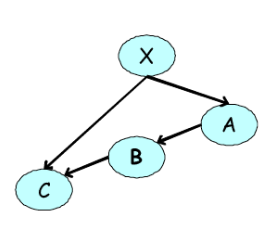
\includegraphics[width=0.3\linewidth]{figures/week_4_2.png}
	\end{figure}
	\begin{align}
		p(A, B, C) &=\sum_{X} p(X) p(A | X) p(B | A) p(C | B, X) \\
		&=p(B | A) \underbrace{\sum_{X} p(X) p(A | X) p(C | B, X)}_{\tx{unnormalized}}
	\end{align}
	\begin{definition}
		A \textbf{factor} $\phi$ describes the local relation between random variables, meanwhile, $\int d\phi$ is \ul{not} necessarily one.
	\end{definition}

	\begin{remark}
		Let $X_\ell \subseteq X$ be a group of local random variables, then $p(X_\ell)$ is automatically a factor $\phi(X_\ell)$.
	\end{remark}

	\begin{align}
		p(A, B, C) &=\sum_{X} \underbrace{p(X) p(A | X) p(B | A) p(C | B, X)}_{\tx{from graphical representation}} \\
		&=\sum_{X} \underbrace{\phi(X) \phi(A, X) \phi(A, B) \phi(X, B, C)}_{\tx{factor representation}} \\
		&=\phi(A, B) \sum_{X} \phi(X) \phi(A, X) \phi(X, B, C) \\
		&=\phi(A, B) \underbrace{\tau(A, B, C)}_{\tx{another factor}}
	\end{align}
	
	\subsection{Sum-Product Inference}
	\begin{theorem}
		Consider a graphical model with random variables $X = Y \cup Z$.
		For an random variable $Y$ in a \ul{directed} or \ul{undirected} model, $P(Y)$ can be computed using the \textbf{sum-product}
		\begin{align}
			\tau(Y) = \sum_z \prod_{\phi \in \Phi} \phi({Scope[\phi]\cap Z}, {Scope[\phi] \cap Y})
		\end{align}
		where $\Phi$ is a set of factors.
	\end{theorem}
	
	\begin{remark}
		For \ul{directed models},
		\begin{align}
			\Phi=\left\{\phi_{x_{i}}\right\}_{i=1}^{N}=\left\{p\left(x_{i} | \text { parents }\left(x_{i}\right)\right)\right\}_{i=1}^{N}
		\end{align}
	\end{remark}
	
%	\begin{example}
%		\begin{figure}[H]
%			\centering
%			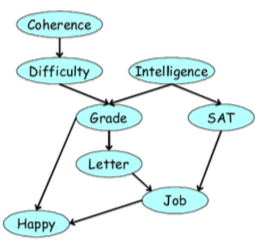
\includegraphics[width=0.3\linewidth]{figures/week_4_3.png}
%		\end{figure}
%		\begin{align}
%			p(C, D, I, G, S, L, H, J)=p(C) p(D | C) p(I) p(G | D, I) p(L | G) P(S | I) p(J | S, L) p(H | J, G)
%		\end{align}
%		using factor representation:
%		\begin{align}
%			\Phi=\{\phi(C), \phi(C, D), \phi(I), \phi(G, D, I), \phi(L, G), \phi(S, I), \phi(J, S, L), \phi(H, J, G)\}
%		\end{align}
%	\end{example}
	
	\subsection{Complexity of Variable Elimination Ordering}
	\begin{theorem}
		The complexity of the variable elimination algorithm is
		\begin{align}
			\mc{O}(m k^{N_{max}})
		\end{align}
		where
		\begin{enumerate}[(i)]
			\item $m$ is the number of initial factors $|\Phi|$;
			\item $k$ is the number of states each random variable takes, assumed to be equal;
			\item $N_i$ is the number of random variables within each summation;
			\item $N_{max} = \max_i N_i$.
		\end{enumerate}
	\end{theorem}
	
	\section{Message passing, Hidden Markov Models, and Sampling}

	\subsection{Message Passing (Computing All Marginals)}
	
	\begin{notation}
		Let $T$ denote the set of edges in a tree. For a node $i$, let $N(i)$ denote the set of its neighbours.
	\end{notation}
	
	The factor of all random variables can be computed following
	
	\begin{align}
		P\left(X_{1: n}\right)
		=\frac{1}{Z} \underbrace{\left[ \prod_{i=1}^n \phi\left(x_{i}\right)
		\right]}_\tx{prior factors}
		\underbrace{\prod_{(i, j) \in T} \phi_{i, j}\left(x_{i}, x_{j}\right)}_\tx{local factors}
	\end{align}
	
	\begin{definition}
		The \textbf{message} sent from variable $j$ to $i \in N(j)$ is
		\begin{align}
			m_{j \rightarrow i}\left(x_{i}\right)
			=\sum_{x_{j}}
			\left [
			\phi_{j}\left(x_{j}\right) \phi_{i j}\left(x_{i}, x_{j}\right)
			\prod_{k \in N(j) \neq i} m_{k \rightarrow j}\left(x_{j}\right)
			\right ]
		\end{align}
	\end{definition}
	
	\begin{algorithm}[Belief Propagation Algorithm]
		Given a tree, inference on an arbitrary node $p(x_i)$ can be computed following:
		\begin{enumerate}
			\item Choose root $r$ arbitrarily;
			\item Pass messages from leaves to $r$;
			\item Pass messages from $r$ to leaves;
			\item Compute inference
			\begin{align}
				p\left(x_{i}\right) \propto \phi_{i}\left(x_{i}\right) \prod_{j \in N(i)} m_{j \rightarrow i}\left(x_{i}\right)
			\end{align}
		\end{enumerate}
	\end{algorithm}
	
	\subsection{Markov Chains}
	\par Using chain rule of probability:
	\begin{align}
		p\left(x_{1: T}\right)=\prod_{t=1}^{T} p\left(x_{t} | x_{t-1}, \ldots, x_{1}\right)
	\end{align}
	
	\begin{definition}
		A Markov chain is said to be \textbf{first-order} if 
		\begin{align}
			p\left(x_{t} | x_{1: t-1}\right)=p\left(x_{t} | x_{t-1}\right)
		\end{align}
	\end{definition}
	
	\paragraph{Simplification} Therefore, for all first-order Markov chains, the full joint distribution can be reduced to
	\begin{align}
		p\left(x_{1: T}\right)=\prod_{t=1}^{T} p\left(x_{t} | x_{t-1}\right)
	\end{align}
	
	\begin{definition}
		A Markov chain is at $m$-order if
		\begin{align}
			p\left(x_{t} | x_{1: t-1}\right)=p\left(x_{t} | x_{t-m: t-1}\right)
		\end{align}
	\end{definition}
	
	\begin{definition}
		A Markov chain is said to be \textbf{homogenous} (i.e., stationary) if
		\begin{align}
			p\left(x_{t} | x_{t-1}\right)=p\left(x_{t+k} | x_{t-1+k}\right) \quad \forall t, k
		\end{align}
	\end{definition}
	
	\paragraph{Parameterization} Assume the random variable $X_t$ takes $k$ states, further suppose the chain is time homogenous. Then characterizing the transition probability
	\begin{align}
		p(x_t | x_{t-1}, x_{t-2}, \cdots, x_{t-m})
	\end{align}
	requires $(k-1) k^m$ parameters.
	
	\subsection{Hidden Markov Models}
	\begin{figure}[H]
		\centering
		\begin{tikzpicture}
		\tikzset{vertex/.style = {shape=circle,draw,minimum size=1.5em}}
		\tikzset{edge/.style = {->,> = latex'}}
		% vertices
		\node[vertex] (x1) at  (0,0) {$x_1$};
		\node[vertex] (z1) at  (0,2) {$z_1$};
		
		\node[vertex] (x2) at  (3,0) {$x_2$};
		\node[vertex] (z2) at  (3,2) {$z_2$};

		\node[vertex] (x3) at  (6,0) {$x_3$};
		\node[vertex] (z3) at  (6,2) {$z_3$};
		
		\node[vertex] (z4) at  (9,2) {$z_{t \geq 4}$};
		%edges
		% Iter 1
		\draw[edge] (z1) to (x1);
		\draw[edge] (z1) to (z2);
		\draw[edge] (z2) to (x2);
		\draw[edge] (z2) to (z3);
		\draw[edge] (z3) to (x3);
		\draw[edge] (z3) to (z4);
		\end{tikzpicture}
		\caption{Hidden Markov Model}
	\end{figure}
	
	\paragraph{Joint distribution} Following the conventional expansion
	\begin{align}
		p(x_{1:T}, z_{1:T}) = p(z_1) \prod_{t=2}^T p(z_t|z_{t-1}) \prod_{t=1}^T p(x_t|z_t)
	\end{align}
	
	\paragraph{Parameterization} Assuming the HMM is \ul{homogenous} with order 1, then the set of parameters $\Phi$ consists of
	\begin{enumerate}[(i)]
		\item Initial distribution of $p(z_1)$: $k-1$ parameters;
		\item Transition distribution of $p(z_{t+1}|z_t)$: $(k-1)k$ parameters;
		\item Emission distribution of $p(x_t|z_t)$: $(k-1)k$ parameters.
	\end{enumerate}
	
	\subsection{Forward-backward Algorithm}
	\paragraph{Smoothing} compute posterior over \ul{past} hidden state
		\begin{align}
			p(z_\tau|x_{1:t})\ s.t.\ 1 < \tau < t
		\end{align}
	\paragraph{Filtering} compute posterior over \ul{current} hidden state
		\begin{align}
			p(z_t|x_{1:t})
		\end{align}
	\paragraph{Prediction} compute posterior over \ul{future} hidden state
		\begin{align}
			p(z_\tau|x_{1:t})\ s.t.\ \tau > t
		\end{align}
	
	\subsection{Procedure of Smoothing (Forward-backward Algorithm)}
	\begin{align}
		p(z_t | x_{1:T})
		&\propto p(x_{1:T}, z_t) \\
		&= p(z_t, x_{1:t}) p(x_{t+1:T}|z_t, x_{1:t}) \\
		&= p(z_t, x_{1:t}) p(x_{t+1:T}|z_t) \\
		&= p(z_t | x_{1:t}) p(x_{1:t}) p(x_{t+1:T}|z_t) \\
		&\propto  p(z_t | x_{1:t}) p(x_{t+1:T}|z_t)
	\end{align}
	
	\paragraph{Forward filtering (encoding)}
	Define
	\begin{align}
		\alpha_t(z_t) := p(z_t|x_{1:t})
	\end{align}
	Then
	\begin{align}
		\red{p(z_t | x_{1:t})}
		&\propto p(z_t, x_{1:t}) \\
		&= \sum_{z_{t-1}=1}^k p(z_{t-1}, z_t, x_{1:t}) \\
		&= \sum_{z_{t-1}=1}^k p(x_t|z_{t-1}, z_t, x_{1:t-1}) p(z_t | z_{t-1}, x_{1:t-1}) p(z_{t-1}, x_{1:t-1}) \\
		&= \sum_{z_{t-1}=1}^k p(x_t|z_t) p(z_t | z_{t-1}) p(z_{t-1}, x_{1:t-1}) \\
		&= p(x_t|z_t) \sum_{z_{t-1}=1}^k p(z_t | z_{t-1}) p(z_{t-1}, x_{1:t-1}) \\
	\end{align}
	Therefore, we have the forward recursion:
	\begin{align}
		\alpha_t(z_t) &= p(x_t|z_t) \sum_{z_{t-1}=1}^k p(z_t | z_{t-1}) \alpha_{t-1}(z_{t-1}) \\
		\alpha_1(z_1) &= p(x_1, z_1)
	\end{align}
	
	\paragraph{Backward filtering (decoding)}
	Define
	\begin{align}
		\beta_t(z_t) = p(x_{t+1:T}|z_t)
	\end{align}
	Then,
	\begin{align}
		p(x_{t+1:T}|z_t)
		&= \sum_{z_{k+1}=1}^k p(x_{t+1:T}, z_{t+1}|z_t) \\
		&= \sum_{z_{k+1}=1}^k p(x_{t+1}, x_{t+2:T}, z_{t+1}|z_t) \\
		&= \sum_{z_{k+1}=1}^k p(x_{t+2:T}, z_{t+1}|z_t, x_{t+1}) p(x_{t+1}|z_t) \\
		&= \sum_{z_{k+1}=1}^k p(x_{t+2:T}, z_{t+1}|z_t, x_{t+1}) p(x_{t+1}|z_t) \\
		&= \sum_{z_{k+1}=1}^k p(x_{t+2:T}, z_{t+1}|z_t) p(x_{t+1}|z_t) \\
		&= \sum_{z_{k+1}=1}^k p(x_{t+2:T}|z_t, z_{t+1}) p(z_{t+1}|z_t) p(x_{t+1}|z_t) \\
		&= \sum_{z_{k+1}=1}^k p(x_{t+2:T}|z_{t+1}) p(z_{t+1}|z_t) p(x_{t+1}|z_t) \\
		&= \sum_{z_{k+1}=1}^k \beta_{t+1}(z_{t+1}) p(z_{t+1}|z_t) p(x_{t+1}|z_t)
	\end{align}

	\subsection{Sampling}
	\paragraph{Problem 1} Generate samples
	\begin{align}
		\{x^{(r)}\}_{r=1}^R \sim p(x)
	\end{align}
	
	\paragraph{Problem 2} Estimate expectations of functions $f(x)$ taking random variable $x \sim p(x)$.
	\begin{align}
		\expe_{x \sim p(x)} f(x) &= \int f(x) p(x)\ dx \\
		&\approx \hat{E} = \frac{1}{N} \sum_{i=1}^N f(x\upi)
	\end{align}
	
	\paragraph{Ancestral sampling} sampling in a topological order. At each step, sample from any conditional distribution that you haven't visited yet, whose parents have all been sampled. This procedure will always start with the nodes that have no parents (i.e., a root).
	
	\paragraph{Generating marginal samples} for nodes $Y \subseteq X$:
	\begin{enumerate}[(i)]
		\item Construct $p(X) = \prod_{x_i \in X} p(x_i|\tx{parent}[x_i])$;
		\item Sample $(x_1, x_2, \cdots, x_N) \sim p(X)$;
		\item Ignore $x_i \notin Y$.
	\end{enumerate}
	
	\paragraph{Generating conditional samples} for nodes $Y \subseteq Xt$ conditioned on $Z \subseteq X$:
	
	\begin{definition}
		The \textbf{simple Monte Carlo} estimator $\hat{\Phi}$ is defined as
		\begin{align}
			\frac{1}{R} \sum_{r=1}^{R} f\left(x^{(r)}\right)=\hat{E} \approx E=\underset{x \sim p(x)}{\mathbb{E}}[f(x)]
		\end{align}
	\end{definition}
	
	\begin{proposition}
		If the sample $\{x^{(r)}\}_{r=1}^R$ are generated from $p(x)$, then $\hat{E}$ is an unbiased estimator of $E$.
	\end{proposition}
	
	\begin{proof}
		\begin{align}
			\mathbb{E}[\hat{E}]_{x \sim p\left(\left\{x^{(i)}\right\}_{r=1}^{R}\right)}
			&= \mathbb{E}\left[\frac{1}{R} \sum_{r=1}^{R} f\left(x^{(r)}\right)\right] \\
			&= \frac{1}{R} \sum_{r=1}^R \expect{f(x^{(r)})} \\
			&= \frac{1}{R} \sum_{r=1}^{R} \expe_{x \sim p(x)}[f(x)] \\
			&= \frac{R}{R} \expe_{x \sim p(x)}[f(x)] \\
			&= E
		\end{align}
	\end{proof}
	
	\begin{proposition}
		As the number of samples of $R$ increases, the variance of $\hat{E}$ will decrease proportional to $\frac{1}{R}$.
	\end{proposition}
	
	\begin{proof}
		\begin{align}
			Var[\hat{E}] &= Var[\frac{1}{R} \sum_{r=1}^R f(x^{(r)})] \\
			&= \frac{1}{R^2} Var[\sum_{r=1}^R f(x^{(r)})] \\
			&= \frac{1}{R^2} \sum_{r=1}^R Var[f(x^{(r)})] \\
			&= \frac{1}{R^2} R Var[f(x)] \\
			&= \frac{1}{R} Var[f(x)]
		\end{align}
	\end{proof}
%	\section{Sampling and Monte Carlo Methods}

	\section{True Skill}
	\par Let $z_i \in \R$ denote player's skill such that
	\begin{align}
		z_i \sim \mc{N}(0, 1)
	\end{align}
	And skills of players are independent such that
	\begin{align}
		p(z_{1:n}) = \prod_{i=1}^np(z_i)
	\end{align}
	Therefore, the joint distribution of skills can be written as a multivariate Gaussian distribution. \\
	Let $X_j$ player $A$ beats player $B$, then
	\begin{align}
		p(\tx{A beat B}|z_A, z_B) = \sigma(z_A - z_B)
	\end{align}
	where $\sigma = 1 / (1 + \exp(z))$. \\
	Then,
	\begin{align}
		p(z_1, z_2 | \tx{A beat B}) \propto p(z_1, z_2) p(\tx{A beat B}|z_1, z_2)
	\end{align}
	\paragraph{Question 1} What's the chance that player A is better than player B in game $\mc{G}$?
	\begin{align}
		p(z_A > z_B|\mc{G}) &= \expe_{p(z_A, z_B|\mc{G})} \id{z_A > z_B} \\
		&\approx  \frac{1}{K} \sum_{i=1}^K \id{z_A > z_B}\quad z_A, z_B \sim p(z_A, z_B|\tx{data}) 
	\end{align}
	
	\begin{figure}[H]
		\centering
		\begin{tikzpicture}
		\tikzset{vertex/.style = {shape=circle,draw,minimum size=1.5em}}
		\tikzset{edge/.style = {->,> = latex'}}
		\node[vertex] (z1) at  (0,0) {$z_1$};
		\node[vertex] (x12) at  (1,-1) {$x_{12}$};
		\node[vertex] (z2) at  (2,0) {$z_2$};
		\node[vertex] (x23) at  (3,-1) {$x_{23}$};
		\node[vertex] (z3) at  (4,0) {$z_3$};
		\node[vertex] (zn) at  (8,0) {$z_N$};
		
		\node[vertex] (x1n) at  (1,-3) {$x_{1N}$};
		
		\node[vertex] (x3n) at  (7,-3) {$x_{3N}$};
		
		\draw[edge] (z1) to (x12);
		\draw[edge] (z2) to (x12);
		\draw[edge] (z2) to (x23);
		\draw[edge] (z3) to (x23);
		
		\draw[edge] (z1) to (x1n);
		\draw[edge] (zn) to (x1n);
		
		\draw[edge] (z3) to (x3n);
		\draw[edge] (zn) to (x3n);
		\end{tikzpicture}
		\caption{Structure of Games}
	\end{figure}
	
	\paragraph{Approximate Inferences} We have $p(z), p(x|z)$ and $x$ (data). \\
	Wish to compute
	\begin{align}
		q(z|x) \approx p(z|x)
	\end{align}
	
	\paragraph{Intractability}
	\begin{align}
		p(z_1|x) &= \int_\R p(z_1, z_2 | x)\ dz_2 \\
		&= \frac{
		\int_\R p(z_1, z_2, x)\ dz_2
		}{
		\iint_{\R^2} p(z_1, z_2, x)\ dz_2\ dz_1
		}
	\end{align}
	
	\subsection{Variational Inferences}
	\paragraph{General Idea of Variational / Approximate Inferences}
	\begin{enumerate}[(i)]
		\item Introduce a tractable \textbf{variational family} $q_\varphi (z | x)$ parameterized using $\varphi$, for example:
		\begin{align}
			q_\varphi (z | x) = \mc{N}(z | \mu_\varphi, \Sigma_\varphi)
		\end{align}
		\item Define \ul{distance} (not necessary a metric) between $p(z|x)$ and $q(z|x)$.
		\item Optimize $\varphi$ to minimize distance, that is,
		\begin{align}
			\expe_{z \sim p(z|x)}[f(z)] \approx \expe_{z \sim q(z|x)}[f(z)]
		\end{align}
	\end{enumerate}
	
	\subsection{Kullback–Leibler Divergence}
	\begin{definition}
		Let $q$ and $p$ be density functions of two distributions $Q$ and $P$, then the \textbf{KL divergence} between $Q$ and $P$ is defined as
		\begin{align}
			KL(q || p) &:= \expe_{q} \left(\log{\frac{q}{p}} \right) \\
			&= \int q(z) \left( \log q(z) - \log p(z) \right)\ dz
		\end{align}
	\end{definition}
	\paragraph{Properties of KL divergence}
	\begin{align}
		KL(q || p) &\geq 0\ \forall p, q \in \Delta(\mc{X}) \\
		KL(q || p) &= 0 \iff p = q \\
		KL(q || p) &\neq KL(p || q) \tx{ in general}
	\end{align}
	\paragraph{Reverse-KL Information Projection} while comparing two distributions, $D_{KL}(q||p) = \expe_q \log \frac{q}{p}$ penalizes (i.e., becomes large) when there are points such that $q \gg p$.
	
	\paragraph{Forward-KL Moment Projection} $D_{KL}(p||q)$ penalizes points when $p \gg q$.
	
	\subsection{Stochastic Variational Inference}
	\paragraph{Evidence Lower Bound} Suppose we are trying to approximate $p(z|x)$ using variational family $q_\varphi(z|x)$. Define
	\begin{align}
		D_{KL}(q_\varphi(z|x) || p(z|x)) 
		&= \expe_{q_\varphi(z|x)} \left[
		\log q_\varphi(z|x) - \log p(z|x)
		\right] \\
		&= \expe_{q_\varphi(z|x)} \left[
		\log q_\varphi(z|x) - \log \frac{p(z, x)}{p(x)}
		\right] \\
		&= \expe_{q_\varphi(z|x)} \left[
		\log q_\varphi(z|x) - \log p(z, x) + \log p(x)
		\right] \\
		&= \expe_{q_\varphi(z|x)} \left[
		\log q_\varphi(z|x) - \log p(z, x) \right]
		+ \expe_{q_\varphi(z|x)} \left[ \log p(x)
		\right] \\
		&= \underbrace{\expe_{q_\varphi(z|x)} \left[
		\log q_\varphi(z|x) - \log p(z, x) \right]}_{-\mc{L}(\varphi;x)}
		+ \underbrace{\log p(x)}_{\perp \varphi}
	\end{align}
	where $\mc{L}(\varphi; x)$ is often referred to as the evidence/empirical lower bound (ELBO). Therefore,
	\begin{align}
		D_{KL}(q_\varphi(z|x) || p(z|x)) &= - \mc{L}(\varphi;x) + \log p(x) \\
		\implies \mc{L}(\varphi;x) + D_{KL}(q_\varphi(z|x) || p(z|x)) &= \log p(x)\quad (\dagger) \\
		\implies \mc{L}(\varphi; x) &\leq \log p(x)
	\end{align}
	Hence, $\mc{L}(\varphi; x)$ is the lower bound of evidence $x$. \ul{By ($\dagger$), maximizing ELBO and minimizing KL divergence are equivalent.}
	
	\paragraph{Re-parameterization Tricks} In order to maximize ELBO, we want to compute the gradient of ELBO with respect to $\varphi$:
	\begin{align}
		\nabla_\varphi \mc{L}(\varphi; x)
		&= \nabla_\varphi \expe_{z \sim q_\varphi(z|x)} [
		\log p(z, x) - \log q_\varphi(z|x)]
	\end{align}
	
	\paragraph{Pathwise Gradient} More generally, let $f$ be an arbitrary function, in our case, $f(z) = \log q_\varphi(z|x) - p(z, x)$. The gradient is
	\begin{align}
		\nabla_\varphi \expe_{q_\varphi(z)} f(z) &= \nabla_\varphi \int q_\varphi(z) f(z)\ dz \\
		&= \int \nabla_\varphi q_\varphi(z) f(z)\ dz\ (\dagger)\tx{ assuming continuity}
	\end{align}
	But $(\dagger)$ is not an expectation, so we cannot use Monte Carlo. \\
	We can exchange differential operator and expectation only if the expectation is independent from $\varphi$. \\
	So we need to factor out the randomness in $f$ from $q_\varphi$, and put it into a parameterless form. That is, we have to
	\ul{re-parameterize using another random variable $\varepsilon$ such that the expectation does not depend on $\varphi$}. \\
	Find $p(\varepsilon)$ and $T(\varepsilon, \varphi)$ such that
	\begin{align}
		\begin{cases}
			\varepsilon \sim p(\varepsilon) \\ 
			z = T(\varepsilon, \varphi)
		\end{cases}
		\implies z \sim q_\varphi(z)
	\end{align}
	
	\begin{example}
		For instance, if we are trying to re-parameterize $q_{\varphi\equiv(\mu, \sigma)} = \mc{N}(\mu, \sigma^2)$ using a standard Gaussian noise $\mc{N}(0, 1)$.
		\begin{align}
			\varepsilon \sim p(\varepsilon) &= \mc{N}(0, 1) \\
			z = T(\varepsilon, \varphi) &= \sigma \varepsilon + \mu
		\end{align}
		so that $z \sim \mc{N}(\mu, \sigma^2)$.
	\end{example}
	
	Using the re-parameterization trick, the gradient can be computed as
	\begin{align}
		\nabla_\varphi \mc{L}(\varphi; x)
		&= \nabla_\varphi \expe_{z \sim q_\varphi(z|x)} [\log p(z, x) - \log q_\varphi(z|x)] \\
		&= \nabla_\varphi \expe_{z \sim q_\varphi(z|x)} [\log p(T(\varepsilon, \varphi), x) - \log q_\varphi(T(\varepsilon, \varphi)|x)] \\
		&= \nabla_\varphi \expe_{\varepsilon \sim p(\varepsilon)} [\log p(T(\varepsilon, \varphi), x) - \log q_\varphi(T(\varepsilon, \varphi)|x)]
	\end{align}
	where the last step holds because the only source of randomness in the expression comes from $\varepsilon$. Since the expectation is no longer depending on $\varphi$, and we can therefore exchange the order of differentiation and expectation:
	\begin{align}
		\nabla_\varphi \mc{L}(\varphi; x)
		&= \expe_{\varepsilon \sim p(\varepsilon)} \nabla_\varphi [\log p(T(\varepsilon, \varphi), x) - \log q_\varphi(T(\varepsilon, \varphi)|x)]
	\end{align}
	
	\paragraph{Stochastic/Automatic Differentiation Variational Inference} As long as we code up
	\begin{align}
		T(\epsilon, \varphi), \log p(x|z), \log p(z), \log q_\varphi (z|x)
	\end{align}
	We can use automatic differentiation techniques to compute gradient
	\begin{align}
		\nabla_\varphi [\log p(T(\varepsilon, \varphi), x) - \log q_\varphi(T(\varepsilon, \varphi)|x)
	\end{align}
	Then estimate the expectation of gradient by Monte Carlo:
	\begin{align}
		\expe_{p(\varepsilon)} \nabla_\varphi \left[
		\log p(x,T(\varepsilon , \varphi)) - \log q_\varphi (T(\varepsilon, \varphi)|x)
		\right] 
		&\approx \frac{1}{K} \sum_{i=1}^K \nabla_\varphi \left[
		\log p(x,T(\varepsilon , \varphi)) - \log q_\varphi (T(\varepsilon, \varphi)|x)
		\right]
	\end{align}
	
	\paragraph{Interpretation of ELBO}
	
	\paragraph{Reinforce / Score Function Estimation} Another method to estimate $- \nabla_\varphi \expe_{q_\varphi(z|x)} L(\varphi)$.\\
	Want
	\begin{align}
		&\nabla_\varphi \expe_{q_\varphi(z)} [f(z)] \\
		&= \nabla_\varphi \int q_\varphi(z) f(z)\ dz \\
		&= \int \nabla_\varphi q_\varphi(z) f(z)\ dz \\
		&= \int f(z) \nabla_\varphi q_\varphi(z) \ dz
	\end{align}
	Note that
	\begin{align}
		\nabla_\varphi \log q_\varphi(z) &= \frac{\nabla_\varphi q_\varphi(z)}{q_\varphi(z)}
	\end{align}
	Therefore,
	\begin{align}
		&\int f(z) \nabla_\varphi q_\varphi(z) \ dz \\
		&= \int f(z) q_\varphi(z) \nabla_\varphi \log q_\varphi(z) \ dz \\
		&= \expe_{q_\varphi(z)}[ f(z) \nabla_\varphi \log q_\varphi(z)]
	\end{align}
	
	\paragraph{Mean-Field Variational Inference}
	\begin{align}
		q(z_1, \cdots, z_N|x) = \prod_{i=1}^N q(z_i|x)
	\end{align}

	\paragraph{Jensen's Inequality}
	\begin{theorem}
		If $f$ is convex, then
		\begin{align}
			f(\expect{X}) \leq \expect{f(x)}
		\end{align}
	\end{theorem}
	Using Jensen's inequality,
	\begin{align}
		\log p_\theta(x) &= \log \int p_\theta(x, z)\ dz \\
		&= \log \int p_\theta(x,z) \frac{q_\varphi(z|x)}{q_\varphi(z|x)}\ dz \\
		&= \log \expe_{q_\varphi(z|x)} \int \frac{p_\theta(x,z)}{q_\varphi(z|x)}\ dz \\
		&\geq \expe_{q_\varphi(z|x)} \int \log \frac{p_\theta(x,z)}{q_\varphi(z|x)}\ dz \\
		&\equiv ELBO(\theta, \varphi)
	\end{align}
	
	\section{Sampling and Monte Carlo Methods}
	\paragraph{Problem} With a target distribution
	\begin{align}
		p(x)
	\end{align}
	and a function
	\begin{align}
		f(x)
	\end{align}
	Wish to compute
	\begin{align}
		\expe_{x \sim p} [f] \equiv \int f(x) p(x)\ dx
	\end{align}
	Note that $\int_{p(x)}$ is rarely analytic, so we have to approximate it. However, drawing samples from $p(x)$ directly is infeasible since we cannot evaluate $p(x)$. Fortunately, we can evaluate $\tilde{p}(x) = Z p(x)$ without knowing $Z$.

	\subsection{Monte Carlo}
	\paragraph{Sampling}
	\begin{align}
		\{x_i\}_{i=1}^R \sim p(x)
	\end{align}
	\paragraph{Simple MC estimator}
	\begin{align}
		\Phi = \expe_{x \sim p(x)}[f] \approx \hat{\Phi} = \frac{1}{R} \sum_{i=1}^R f(x_i)
	\end{align}
	Therefore, Monte Carlo turns estimation problem into a sampling problem.
	Note that MC estimator is unbiased and variance shrinks proportional to $\frac{1}{R}$. \\
	Further, the variance is independent of dimensionality. \\
	Note that sampling from high dimensions is still hard. Why? So far, we've assumed 
	\begin{align}
		p(x) &= \frac{\tilde{p}(x)}{Z} = \frac{\tilde{p}(x)}{\int d\tilde{p}(x)} \\
		p(x) &\propto \tilde{p}(x)
	\end{align}

	\paragraph{Aside} No that $\tilde{p}$ is the joint distribution of $q(pred; data)$. In this case, $p$ could be the likelihood $q(pred|data) = \frac{q(pred, data)}{\int_{pred}dq(pred, data)}$. $Z = p(data)$ is often referred to as the \textbf{evidence}.

	\paragraph{Why is sampling $x \sim p$ hard?} Firstly, in most cases, we don't know the exact value of $Z$, and computing $Z$ by integrating $\tilde{p}$ requires prohibitive computational power. Event if we know $Z$, we wish so sample from $\mc{X}$ where $p(x)$ is large. But for most distributions, we can't do exactly without enumerating all possible $x$, which is challenging when $x$ is in high dimensional spaces.
	
	\paragraph{Easy Distributions?} For some families of distributions like Gaussian distribution, sampling from them can be easy.
	
	\subsubsection{Lattice Discretization (Bad idea!)}
	\begin{algorithm}[Lattice Discretization]\quad
		\begin{enumerate}[(i)]
			\item Discretize $\mc{X}$ into finitely many uniformly spaced points $\{x_i\}$. The collection of points form a lattice of $\mc{X}$.
			\item Evaluate $\tilde{p}(x_i)$ on each point $x_i$.
			\item Estimate normalizing constant $Z \approx \sum_i \tilde{p}(x_i)$.
			\item Estimate probability using $p(x) \approx \frac{\tilde{p}(x)}{Z}$. 
		\end{enumerate}
	\end{algorithm}
	
	\par Using lattice to sample is a bad idea, if the lattice is too coarse, the estimated distribution is biased. If the lattice is too dense, then we're wasting computational resources. Further, the number of points required as well as computational cost grow exponentially as the dimension $\mc{X}$ increases.
	
	\subsection{Monte Carlo Methods for Sampling}
	\subsubsection{Uniform Sampling}
	\subsubsection{Importance Sampling}
	\paragraph{Importance Weight Sampler} Sampling from $p$ is hard, we sample $x^r$ from a simpler distribution $q$ (e.g., $p \sim \mc{N}$) instead. Weight each sample from $q$ by $w_r = \frac{\tilde{p}(x^r)}{q(x^r)}$. Recall that we know how to evaluate the unnormalized density $\tilde{p}$.
	\todo{See more on the next section}
	\subsubsection{Rejection Sampling}
	\paragraph{Rejection Sampling} Assume
	\begin{align}
		\tilde{p}(x) &= p(x) Z_p\ Z_p \in \R \\
		\tilde{q}(x) &= q(x) Z_q\ Z_q \in \R
	\end{align}
	and we can evaluate $\tilde{q}$ cheaply and we can sample from $q$ easily. Further, assume
	\begin{align}
		\exists\ c\ s.t.\ c \tilde{q}(x) > \tilde{p}(x)\quad \forall x
	\end{align}
	\begin{algorithm}[Rejection Sampling] \quad
		\begin{enumerate}[(i)]
			\item Generate two random numbers $(x, u)$.
			\begin{enumerate}[(a)]
				\item Sample $x \sim q$;
				\item Sample $u \sim Unif[0, c \tilde{q}(x)]$;
			\end{enumerate}
			\item Evaluate $\tilde{p}(x)$
			\begin{enumerate}[(a)]
				\item if $u > \tilde{p}(x)$, reject this sample;
				\item Otherwise $x$ is accepted and added to our set of samples $\lbrace x^{(r)} \rbrace$.
			\end{enumerate}
		\end{enumerate}
	\end{algorithm}
	
	\paragraph{Intuition} Note that all samples are independently sampled from an identical distribution. Therefore, probability for a particular value of $x$ to be added to the sample is
	\begin{align}
		Prob(x) &= q(x) Prob(Accept|x) \\
		&= q(x) \frac{\tilde{p}(x)}{c \tilde{q}(x)} \\
		&= \frac{\tilde{p}(x)}{Z_q c} \propto p(x)
	\end{align}
	
	\paragraph{Limitations} For rejection sampling, if the two distributions $p$ and $q$ are not similar, $c$ have to be large so that $c \tilde{q}$ covers $\tilde{q}$ everywhere in $\mc{X}$. A large value fo $c$ makes acceptance rare.
	
	\paragraph{Limitations} The rejection sampling requires $p \approx q$. Otherwise, the $C$ required is large. When $p$ and $q$ are on $D$ dimensions, then $C \in \mc{O}(\exp(\sqrt{D}))$. The acceptance rate is $\frac{1}{C}$ in one dimension, and the rate reduces exponentially in dimension.
	\begin{align}
		\expe_p [f] = \int f(x) p(x)\ dx
	\end{align}
	Since integral is a linear operator, when integrant is large, the expectation is large as well.
	
	\subsubsection{Metropolis-Hastings Method}
	\paragraph{Typical set} Because expectation is a linear operator, all samples that contribute significantly to the $\expe$ come from the typical set. \todo{Check the definition of typical set.}

	\paragraph{Markov Chain Monte Carlo (MCMC)} Stochastically explore the typical set. We need a Markov transition distribution, from which we can sample $x_{t+1}$:
	\begin{align}
		x_{t+1} \sim T(x'|x_t)
	\end{align}
	\begin{proposition} Properties of $T$
		1) $p$ is invariant under $T$:
		\begin{align}
			p(x) = \int T(x|x') p(x')\ dx'
		\end{align}
		2) Ergodic: $p^{(t)} \to p(x)$.
	\end{proposition}
	
	\paragraph{Metropolis} Given background distribution $p$, we only observe $\tilde{p}$ but not $p$. Define $T$ as
	\begin{enumerate}[(i)]
		\item Proposal distribution $q$, which is not necessarily similar to $p$.
		\begin{align}
			x' \sim q(x'|x_t)
		\end{align}
		\item Accept $x'$ as $x_{t+1}$? 
		\begin{align}
			a := \frac{\tilde{p}(x') q(x_t|x')}{\tilde{p}(x_t) q(x'|x_t)}
		\end{align}
		\begin{enumerate}[(a)]
			\item If $a \geq 1$ accept $x_{t+1} \leftarrow x'$.
			\item If $a < 1$, accept $x_{t+1} \leftarrow x'$ with probability $a$; otherwise, reject and set $x_{t+1} \leftarrow x_t$.
		\end{enumerate}
	\end{enumerate}
	
	\paragraph{Random Walk Metropolis}
	\begin{align}
		q(x'|x_t) = \mc{N} (x'|x_t, \sigma^2)
	\end{align}

	\paragraph{Hamiltonian Monte Carlo}
	\begin{align}
		x &\to (x, v) \\
		q(x) &\to q(x, v) = q(x) q(v|x) \\
		H(x, v) &= - \log(q(x, v)) = - \overbrace{\log(q(x))}^{U: PE} - \overbrace{\log(q(v|x))}^{K: KE}
	\end{align}
	
	\subsection{Tutorial on Sampling}
	\paragraph{Problem} Say one wishes to sample 
	\begin{align}
		x \sim p(x) = \frac{\tilde{p}(x)}{Z}
	\end{align}
	such that
	\begin{align}
		\int p(x)\ dx &= 1 \\
		\int \tilde{p}(x)\ dx &= Z \\
		\tilde{p}(x), p(x) &\geq 0
	\end{align}

	\paragraph{Goal} For an arbitrary function $\phi$, we wish to estimate
	\begin{align}
		\expe_{x \sim p(x)} \phi(x) = \int p(x) \phi(x)\ dx
	\end{align}
	by sampling $x \sim p(x)$.

	\paragraph{Challenge} We only observe the potential $\tilde{p}(x)$ but not the actual probability $p(x)$. In addition, marginalizing the potential (i.e., computing $\int_x \tilde{p}(x)\ dx$) is prohibitive, so that one may \ul{not} reconstruct the probability $p(x)$ directly.

	\paragraph{Cheap Sampling} We may assume sampling from a certain class of distributions to be cheap. For instance, we can sample from a Gaussian distribution cheaply:
	\begin{align}
		x \sim \mc{N}(\mu, \sigma^2)
	\end{align}
	
	\paragraph{Idea} For most of sampling techniques covered in this course, we are sampling from an "auxiliary potential", say $\tilde{q}(x)$, from which we can sample with ease. Then, we estimate $p(x)$ via sampling result from $\tilde{q}$ and our knowledge on $\tilde{p}$.
	
	\subsubsection{Importance Sampling}
	\paragraph{Problem} Suppose
	\begin{align}
		\tilde{p}(x) &= Z_p p(x) \\
		\tilde{q}(x) &= Z_q q(x)
	\end{align}
	where the normalizing constants are unknown. And we wish to estimate 
	\begin{align}
		\expe_{x \sim p(x)} \phi(x)
	\end{align}
	for some function $\phi$.

	\paragraph{Solution} We may take $\tilde{q}(x) = \mc{N}(\mu, \sigma^2)$, in this case, $Z_q = 1$.
	
	\info{[?] Do we know both $\tilde{q}$ and $Z_q$ or we only know $q$?}
	\begin{algorithm}[Importance Sampling] \quad
		\begin{enumerate}[(i)]
			\item Sample $X^{1:R} \sim Z_q q(x)= \tilde{q}(x)$.
			\item Estimate expectation under $q$: $\expe_{q}(\phi(x)) \approx \frac{1}{R} \sum_{i=1}^R \phi(x_i)$.
			\item Weight each sample using \ul{importance weights} $\tilde{w}_i = \frac{\tilde{p}(x_i)}{\tilde{q}(x_i)}$.
		\end{enumerate}
	\end{algorithm}
	
	\paragraph{Intuition} For one particular sample $x$, if $\tilde{p}(x) > \tilde{q}(x)$, $\tilde{p}$ is \ul{underrepresented while sampling using $\tilde{q}$}, so we assign this sample with larger weight $w$.
	
	\paragraph{Estimation} Recall that the ultimate goal of sampling exercises is to estimate $\expe_p \phi(x)$:
	\begin{align}
		\expe_p \phi(x) &= \int p(x) \phi(x)\ dx \\
		&= \int q(x) \frac{p(x)}{q(x)} \phi(x)\ dx \\
		&= \expe_q \frac{p(x)}{q(x)} \phi(x) \\
		&\approx \frac{1}{R} \sum_{i=1}^R \underbrace{\frac{p(x_i)}{q(x_i)}}_{(\dagger)} \phi(x_i) \tx{ where } x_i \sim q(x)
	\end{align}
	Note that we only have the unnormalized version of $(\dagger)$, therefore,
	\begin{align}
		... &= \frac{1}{R} \sum_{i=1}^R \frac{\tilde{p}(x_i)/Z_p}{\tilde{q}(x_i)/Z_q} \phi(x_i) \\
		&= \frac{Z_q}{Z_p} \frac{1}{R} \sum_{i=1}^R \frac{\tilde{p}(x_i)}{\tilde{q}(x_i)}\phi(x_i) \\
		&= \frac{Z_q}{Z_p} \frac{1}{R} \sum_{i=1}^R \tilde{w}_i \phi(x_i)\quad (\dagger \dagger)
	\end{align}
	\begin{lemma}
		\begin{align}
			\sum_{i=1}^R \tilde{w}_i
			&= \sum_{i=1}^R \frac{\tilde{p}(x_i)}{\tilde{q}(x_i)}
			= \sum_{i=1}^R \frac{\tilde{p}(x_i) \frac{Z_q}{Z_p}}{\tilde{q}(x_i) \frac{Z_q}{Z_p}} \tx{ where } x_i \sim q(x) \\
			&= \sum_{i=1}^R \frac{p(x_i) Z_q}{\tilde{q}(x_i) \frac{Z_q}{Z_p}} 
			= \sum_{i=1}^R \frac{p(x_i) Z_q}{q(x_i) Z_q \frac{Z_q}{Z_p}} \\
			&= \sum_{i=1}^R \frac{p(x_i)}{q(x_i) \frac{Z_q}{Z_p}}
			= \frac{Z_p}{Z_q} \sum_{i=1}^R \frac{p(x_i)}{q(x_i)} \\
			&= R \frac{Z_p}{Z_q} \frac{1}{R} \sum_{i=1}^R \frac{p(x_i)}{q(x_i)} \\
			&\overset{R \to \infty}{=} R \frac{Z_p}{Z_q} \expe_q \frac{p(x)}{q(x)} \\
			&= R \frac{Z_p}{Z_q} \int_\R q(x) \frac{p(x)}{q(x)}\ dx
			= R \frac{Z_p}{Z_q}
		\end{align}
		Therefore, 
		\begin{align}
			\frac{Z_p}{Z_q} &= \frac{1}{R} \sum_{i=1}^R \tilde{w}_i
		\end{align}
	\end{lemma}
	Hence,
	\begin{align}
		\expe_p \phi(x) \approx (\dagger \dagger) = \frac{\sum_{i=1}^R \tilde{w}_i \phi(x_i)}{\sum_{i=1}^R \tilde{w}_i}
	\end{align}
\end{document}




























